%%%%%%%%%%%%%%%%%%%%%%%%%%%%%%%%%%%%%%%%%%%%%%
%                insertmeeting
% 1) Title (something creative & funny?)
% 2) Date (MM/DD/YYYY)
% 3) Location (ex. Hagerty High School)
% 4) People/Committees Present 
% 5) Picture 
% 6) Start Time & Stop Time (ex. 12:30AM to 4:30PM)
%%%%%%%%%%%%%%%%%%%%%%%%%%%%%%%%%%%%%%%%%%%%%%
\insertmeeting 
	{All Eyes on Me} 
	{01/21/22} 
	{Hagerty High School}
	{Clayton, Falon, James, Jensen, Nathan, Ritam, Rose, Samantha}
	{Images/RobotPics/robot.jpg}
	{2:30 - 4:30}
	
\hhscommittee{Software}
\noindent\hfil\rule{\textwidth}{.4pt}\hfil
\subsubsection*{Goals}
\begin{itemize}
    \item Start a new OpenCV pipeline to identify the carousel post 

\end{itemize} 

\noindent\hfil\rule{\textwidth}{.4pt}\hfil

\subsubsection*{Accomplishments}
In Tele-Op, we have experienced difficulty navigating accurately to the carousel. One solution we decided to explore today was finding the colored pole of the carousel using OpenCV, and receiving positional data from that. To accomplish this, we used a program called GRIP. The software allowed us to test various configurations of image manipulation and computer vision techniques to refine the input. We used a picture of the carousel taken by a phone as a test image. At first, we tried to grayscale the image and use an adaptive threshold. However, the software was unable to differentiate the colored pole from the background due to the shadow from the carousel. We then attempted to improve the quality of the image through erosions and dilations. However, this method still suffered from the shadow on the carousel. So, we decided to switch to using an HSV threshold, combined with the erosions and dilations. This produced a usable image. In the future, we have to focus on refining the HSV threshold of the pipeline and calculating the correct contour. We can do this by drawing rectangles on the image and saving them into the control hub. 


\hhscommittee{Software}
\noindent\hfil\rule{\textwidth}{.4pt}\hfil
\subsubsection*{Goals}
\begin{itemize}
    \item Start a new OpenCV pipeline to identify the carousel post 

\end{itemize} 

\noindent\hfil\rule{\textwidth}{.4pt}\hfil

\subsubsection*{Accomplishments}
Following our last CAD meeting where we CADed our latest intake version, we set up our 2 parts to print out of nylon at UCF. Back at Hagerty with the completed 3D printed parts, we cut out the laser cut parts using our glowforge and were ready to get started putting it together. First we screwed the sweeper arm together and put all of the bearings into the plates. Finding that the holes were a bit too small, so we used a 12mm drill bit to widen them to fit the bearings snugly. Next we screwed the sides onto the nylon intake base from the last version of the intake. Moving on to the sweeper itself, we chase to remain with the rubber flaps. This time however we used the laser cutter to cut them out, ensuring that they would be the exact right length and shape to fit through the holes. Hooking all of these parts together and adding the pulleys and belts, we completed what we hoped would be the final version of the intake until after leagues. While testing it, we found that we needed to add more tension to hold the sweeper arm down, so we connected some rubber bands between the intake base and the sweeper arm. In a similar vein, we added a string between the base and the arm to keep the arm from pivoting up too far and releasing an element. This allows the arm to pivot as we intended without pivoting too far. Upon testing the design, we found that it worked fantastically! Feeling extremely optimistic, we started some driver practice and picked up blocks with ease. The best part was that we could both pick up balls without damaging the servo in any way and we could intake blocks without throwing them when we flip the intak to get ready to score. To see this intake attached and in action, see our marvelous robot, Scoopie!



\begin{figure}[htp]
\centering
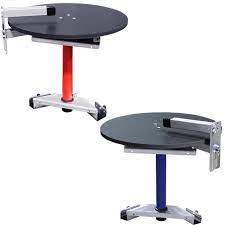
\includegraphics[width=0.95\textwidth, angle=0]{Meetings/January/01-21-22/1.21.22 carousel posts - James Hu.jpeg}
\caption{Images we used while creating the pipeline}
\label{fig:012122_1}
\end{figure}


\whatsnext{
\begin{itemize}
    \item Continue to refine the pipeline and integrate into tele-op. 
    \item Let software work on a cycle auto
	\item Prepare for League champs!

\end{itemize} 
}

